% !TEX program = xelatex
% 编译方式：XeLaTeX（需 ctex 宏包与中文字体；Overleaf 直接上传本文件即可编译）
\documentclass[11pt,a4paper]{article}

% ==================== 宏包 ====================
\usepackage[UTF8]{ctex}
\usepackage{amsmath, amssymb, amsfonts}
\usepackage{geometry}
\geometry{margin=2.3cm}
\usepackage{graphicx}
\usepackage{booktabs}
\usepackage{array}
\usepackage{listings}
\usepackage{xcolor}
\usepackage{hyperref}
\usepackage{caption}
\usepackage{float}
\usepackage{bm}
\usepackage{tikz}
\usetikzlibrary{arrows.meta, positioning, calc}

% ==================== 代码高亮 ====================
\definecolor{codegreen}{rgb}{0.0,0.5,0.35}
\definecolor{codeblue}{rgb}{0.16,0.32,0.75}
\definecolor{codegray}{rgb}{0.45,0.45,0.45}
\definecolor{codebg}{rgb}{0.96,0.97,0.98}

\lstdefinestyle{py}{
    language=Python,
    backgroundcolor=\color{codebg},
    commentstyle=\color{codegreen},
    keywordstyle=\color{codeblue}\bfseries,
    stringstyle=\color{codegray},
    basicstyle=\ttfamily\small,
    breaklines=true,
    numbers=left,
    numberstyle=\tiny\color{codegray},
    numbersep=6pt,
    frame=single,
    rulecolor=\color{codegray!40},
    showstringspaces=false,
    columns=flexible,
    keepspaces=true,
    morekeywords={softmax,layernorm}
}
\lstset{style=py}

\hypersetup{
    colorlinks=true,
    linkcolor=codeblue,
    citecolor=codeblue,
    urlcolor=codeblue
}

\title{\textbf{基于 Transformer 的倒立摆控制}\\[0.5em]
\large 系统建模、最优控制与深度学习控制的完整理论及编码实现}
\author{技术文档}
\date{\today}

\begin{document}
\maketitle

\begin{abstract}
本文完整阐述用 \textbf{Transformer} 神经网络控制倒立摆（Cart--Pole）的理论与实现。内容覆盖四个层面：
\textbf{(i) 系统建模}——从质点杆模型出发，经拉格朗日方程严格推导非线性动力学，再由一阶泰勒展开得到状态空间线性化模型，并分析开环稳定性与可控性；
\textbf{(ii) 最优控制}——由庞特里亚金极小值原理完整导出线性二次型调节器（LQR）的 Riccati 方程，给出离散化迭代求解算法；
\textbf{(iii) 深度学习}——系统讲解 Transformer 的缩放点积注意力、多头注意力、位置编码、前馈网络与残差连接各组件及其数学依据；
\textbf{(iv) 编码实现}——以纯 NumPy 手写物理仿真、LQR 求解、Transformer 前向与反向传播、训练循环，并对每段代码逐行说明。
实验表明，经模仿学习训练的 Transformer 控制器能稳定维持倒立摆平衡，输出与 LQR 专家高度一致。
\end{abstract}

\tableofcontents
\newpage

% ======================================================================
\section{引言}
% ======================================================================

倒立摆系统由可沿水平轨道运动的小车与铰接于小车顶端的摆杆组成，控制目标为施加水平力 $F$，使摆杆维持在竖直向上的\textbf{不稳定平衡点}附近，同时小车位置回归原点。该系统集\textbf{欠驱动}（仅一个控制输入、两个自由度）、\textbf{非线性}、\textbf{开环不稳定}于一身，是控制理论与机器人学的经典验证平台。

控制方法大致沿两条路线演进：

\begin{itemize}
    \item \textbf{基于模型}：PID、LQR、模型预测控制（MPC）。需要建立并线性化模型，控制器结构明确、可解释，但对建模精度敏感。
    \item \textbf{数据驱动}：强化学习、模仿学习。直接从数据学习策略，无需精确模型，但可解释性较弱。
\end{itemize}

Transformer \cite{vaswani2017attention} 凭借\textbf{多头自注意力}在序列建模上取得巨大成功。其本质能力——对序列任意位置间的长程依赖直接建模——与控制问题高度契合：控制器本质上是\textbf{由观测历史到当前动作}的序列决策器。本文将倒立摆控制形式化为序列决策任务，用 Transformer 作为策略网络，经模仿学习训练，并给出从建模到编码的完整闭环。

% ======================================================================
\section{倒立摆系统建模}
% ======================================================================

\subsection{系统描述、坐标系与假设}

图 \ref{fig:cartpole} 为系统示意。设小车质量 $M$，摆杆质量 $m$，摆杆半长（质心到铰点距离）$l$，重力加速度 $g$。广义坐标取小车水平位移 $x$（向右为正）与摆杆偏角 $\theta$（相对竖直向上，顺时针为正）。控制输入为水平力 $F$。

\begin{figure}[H]
\centering
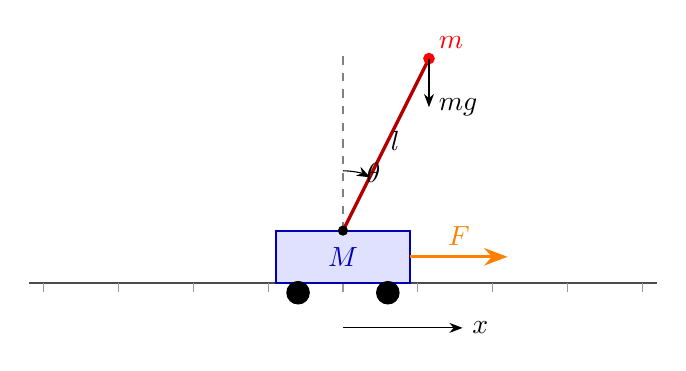
\begin{tikzpicture}[scale=0.95]
  % 地面轨道
  \draw[thick, black!70] (-4.2,0) -- (4.2,0);
  \foreach \i in {-4,-3,...,4}
    \draw[black!40] (\i,0) -- (\i,-0.12);
  % 小车
  \filldraw[fill=blue!12, draw=blue!70!black, thick] (-0.9,0) rectangle (0.9,0.7);
  % 车轮
  \filldraw[black] (-0.6,-0.13) circle (0.15);
  \filldraw[black] (0.6,-0.13) circle (0.15);
  % 竖直参考虚线
  \draw[dashed, gray, thin] (0,0.7) -- (0,3.1);
  % 摆杆（偏角 theta）
  \draw[very thick, red!70!black] (0,0.7) -- (1.15,3.0);
  % 铰点
  \filldraw[black] (0,0.7) circle (0.06);
  % 质心
  \filldraw[red] (1.15,3.0) circle (0.07) node[above right] {$m$};
  % 角度弧
  \draw[-{Stealth}, black] (0,1.5) arc (90:63:0.8) node[midway, right] {$\theta$};
  % 力箭头
  \draw[-{Stealth}, very thick, orange] (0.9,0.35) -- (2.2,0.35) node[midway, above] {$F$};
  % 坐标轴
  \draw[-{Stealth}] (0,-0.6) -- (1.6,-0.6) node[right] {$x$};
  % 质量标注
  \node[blue!70!black] at (0,0.35) {$M$};
  % 杆长标注
  \node[black] at (0.7,1.9) {$l$};
  % 重力
  \draw[-{Stealth}, black] (1.15,3.0) -- (1.15,2.35) node[right] {$mg$};
\end{tikzpicture}
\caption{倒立摆（Cart--Pole）系统示意图：小车质量 $M$、摆杆质量 $m$（质点模型）、半长 $l$、偏角 $\theta$（相对竖直向上）、水平控制力 $F$。}
\label{fig:cartpole}
\end{figure}

\textbf{关键假设（质点杆模型）}：将摆杆质量 $m$ 视为集中于距铰点 $l$ 处的单个质点，忽略杆的转动惯量。该假设使非线性动力学与后续线性化结果\textbf{严格自洽}——若采用均匀杆（绕质心惯量 $ml^2/3$），线性化结果将含有 $\tfrac{4}{3}$ 因子，而本文的质点模型可精确退化为教科书标准形式。参数取值见表 \ref{tab:param}。

\begin{table}[H]
\centering
\caption{系统参数与状态变量}
\label{tab:param}
\begin{tabular}{@{}cll@{}}
\toprule
符号 & 含义 & 取值 \\
\midrule
$M$ & 小车质量 & $1.0\ \mathrm{kg}$ \\
$m$ & 摆杆质量 & $0.1\ \mathrm{kg}$ \\
$l$ & 摆杆半长 & $0.5\ \mathrm{m}$ \\
$g$ & 重力加速度 & $9.81\ \mathrm{m/s^2}$ \\
$x$ & 小车位置 & 状态量 \\
$\theta$ & 摆杆偏角 & 状态量 \\
$F$ & 水平控制力 & 控制输入 \\
\bottomrule
\end{tabular}
\end{table}

\subsection{运动学：质心位置与速度}

摆杆质心在惯性系中的坐标为
\begin{equation}
    x_{\mathrm{cm}} = x + l\sin\theta, \qquad y_{\mathrm{cm}} = l\cos\theta .
\end{equation}
对时间求导得质心速度：
\begin{equation}
    \dot x_{\mathrm{cm}} = \dot x + l\dot\theta\cos\theta, \qquad
    \dot y_{\mathrm{cm}} = -l\dot\theta\sin\theta .
\end{equation}

\subsection{拉格朗日量：动能与势能}

系统动能 $T$ 由小车平动与杆质心运动两部分构成：
\begin{equation}
\begin{aligned}
    T &= \underbrace{\frac{1}{2}M\dot x^2}_{\text{小车平动}}
       + \underbrace{\frac{1}{2}m\big(\dot x_{\mathrm{cm}}^2 + \dot y_{\mathrm{cm}}^2\big)}_{\text{杆质心运动}} \\
      &= \frac{1}{2}M\dot x^2 + \frac{1}{2}m\Big[(\dot x + l\dot\theta\cos\theta)^2 + (l\dot\theta\sin\theta)^2\Big] .
\end{aligned}
\end{equation}
展开平方项并利用 $\cos^2\theta + \sin^2\theta = 1$：
\begin{equation}
\begin{aligned}
    T &= \frac{1}{2}M\dot x^2 + \frac{1}{2}m\big(\dot x^2 + 2l\dot x\dot\theta\cos\theta + l^2\dot\theta^2\cos^2\theta + l^2\dot\theta^2\sin^2\theta\big) \\
      &= \frac{1}{2}(M+m)\dot x^2 + ml\,\dot x\dot\theta\cos\theta + \frac{1}{2}ml^2\dot\theta^2 .
\end{aligned}
\end{equation}

以摆杆竖直向下为零势能点，势能为
\begin{equation}
    V = m g\, y_{\mathrm{cm}} = m g l \cos\theta .
\end{equation}

拉格朗日量
\begin{equation}
    \mathcal{L} = T - V = \frac{1}{2}(M+m)\dot x^2 + ml\dot x\dot\theta\cos\theta + \frac{1}{2}ml^2\dot\theta^2 - mgl\cos\theta .
\end{equation}

\subsection{欧拉--拉格朗日方程}

对广义坐标 $q \in \{x, \theta\}$，欧拉--拉格朗日方程为
\begin{equation}
    \frac{\mathrm d}{\mathrm dt}\Big(\frac{\partial \mathcal L}{\partial \dot q}\Big) - \frac{\partial \mathcal L}{\partial q} = Q_q ,
\end{equation}
其中广义力 $Q_x = F$（外力沿 $x$ 方向做功），$Q_\theta = 0$（摆杆无外力矩）。

\paragraph{对 \texorpdfstring{$x$}{x} 方向。} 计算各偏导：
\begin{equation}
    \frac{\partial \mathcal L}{\partial \dot x} = (M+m)\dot x + ml\dot\theta\cos\theta ,
\end{equation}
\begin{equation}
    \frac{\mathrm d}{\mathrm dt}\Big(\frac{\partial \mathcal L}{\partial \dot x}\Big)
    = (M+m)\ddot x + ml\ddot\theta\cos\theta - ml\dot\theta^2\sin\theta ,
\end{equation}
\begin{equation}
    \frac{\partial \mathcal L}{\partial x} = 0 .
\end{equation}
代入得第一个运动方程
\begin{equation}
    \boxed{\; (M+m)\ddot x + ml\ddot\theta\cos\theta - ml\dot\theta^2\sin\theta = F \;}
    \label{eq:eom1}
\end{equation}

\paragraph{对 \texorpdfstring{$\theta$}{θ} 方向。} 同理：
\begin{equation}
    \frac{\partial \mathcal L}{\partial \dot\theta} = ml\dot x\cos\theta + ml^2\dot\theta ,
\end{equation}
\begin{equation}
    \frac{\mathrm d}{\mathrm dt}\Big(\frac{\partial \mathcal L}{\partial \dot\theta}\Big)
    = ml\ddot x\cos\theta - ml\dot x\dot\theta\sin\theta + ml^2\ddot\theta ,
\end{equation}
\begin{equation}
    \frac{\partial \mathcal L}{\partial \theta} = -ml\dot x\dot\theta\sin\theta + mgl\sin\theta .
\end{equation}
代入得第二个运动方程，注意到 $-ml\dot x\dot\theta\sin\theta$ 两项相消：
\begin{equation}
    ml\ddot x\cos\theta + ml^2\ddot\theta - mgl\sin\theta = 0 .
\end{equation}
两边同除以 $ml$：
\begin{equation}
    \boxed{\; \ddot x\cos\theta + l\ddot\theta - g\sin\theta = 0 \;}
    \label{eq:eom2}
\end{equation}

\subsection{显式化：解出 \texorpdfstring{$\ddot\theta$}{θ̈} 与 \texorpdfstring{$\ddot x$}{ẍ}}

式 \eqref{eq:eom1}、\eqref{eq:eom2} 为关于 $\ddot x, \ddot\theta$ 的线性方程组。由式 \eqref{eq:eom1} 解出 $\ddot x$：
\begin{equation}
    \ddot x = \frac{F - ml\ddot\theta\cos\theta + ml\dot\theta^2\sin\theta}{M+m} .
\end{equation}
代入式 \eqref{eq:eom2} 消去 $\ddot x$：
\begin{equation}
    \frac{F\cos\theta + ml\dot\theta^2\sin\theta\cos\theta}{M+m}
    - \frac{ml\cos^2\theta}{M+m}\ddot\theta + l\ddot\theta = g\sin\theta .
\end{equation}
合并 $\ddot\theta$ 项：
\begin{equation}
    \ddot\theta\Big[ l - \frac{ml\cos^2\theta}{M+m}\Big]
    = g\sin\theta - \frac{\cos\theta\,(F + ml\dot\theta^2\sin\theta)}{M+m} .
\end{equation}
最终得到
\begin{equation}
\boxed{\;
    \ddot\theta = \frac{g\sin\theta - \cos\theta\,\dfrac{F + ml\dot\theta^2\sin\theta}{M+m}}
                     {l\Big(1 - \dfrac{m\cos^2\theta}{M+m}\Big)}
\;}
\label{eq:thetadd}
\end{equation}
回代得
\begin{equation}
\boxed{\;
    \ddot x = \frac{F + ml\,(\dot\theta^2\sin\theta - \ddot\theta\cos\theta)}{M+m}
\;}
\label{eq:xdd}
\end{equation}

式 \eqref{eq:thetadd}、\eqref{eq:xdd} 即仿真所用的完整非线性动力学。定义状态向量 $\mathbf z = [x,\ \dot x,\ \theta,\ \dot\theta]^{\top}$ 与输入 $u = F$，得状态方程
\begin{equation}
    \dot{\mathbf z} = f(\mathbf z, u)
    = \begin{bmatrix} \dot x \\ \ddot x \\ \dot\theta \\ \ddot\theta \end{bmatrix} .
\end{equation}

\subsection{平衡点线性化：一阶泰勒展开}

\paragraph{平衡点。} 直立平衡条件为 $\theta = 0,\ \dot\theta = 0,\ \dot x = 0,\ u = 0$。在平衡点邻域做一阶泰勒展开：
\begin{equation}
    \dot{\mathbf z} \approx f(\mathbf z^*, u^*) + \underbrace{\frac{\partial f}{\partial \mathbf z}\Big|_{*}}_{\mathbf A}(\mathbf z - \mathbf z^*) + \underbrace{\frac{\partial f}{\partial u}\Big|_{*}}_{\mathbf B} u .
\end{equation}

\paragraph{求 \texorpdfstring{$\mathbf A$}{A} 与 \texorpdfstring{$\mathbf B$}{B}。} 状态方程中，$f_1 = \dot x$、$f_3 = \dot\theta$ 为恒等式，故 $\mathbf A$ 的第 1、3 行分别为 $[0,1,0,0]$、$[0,0,0,1]$。关键在于 $f_2 = \ddot x$ 与 $f_4 = \ddot\theta$ 的偏导。

先求 $\ddot\theta$ 对 $\theta$ 与 $u$ 的偏导。记式 \eqref{eq:thetadd} 的分子为 $N(\theta, u)$、分母为 $D(\theta)$：
\begin{equation}
    N = g\sin\theta - \frac{\cos\theta\,(u + ml\dot\theta^2\sin\theta)}{M+m},
    \qquad
    D = l\Big(1 - \frac{m\cos^2\theta}{M+m}\Big) .
\end{equation}
在平衡点（$\theta = \dot\theta = u = 0$）处：
\begin{equation}
    \frac{\partial N}{\partial\theta}\Big|_* = g\cos\theta = g, \qquad
    \frac{\partial D}{\partial\theta}\Big|_* = 0, \qquad
    D|_* = l\Big(1-\frac{m}{M+m}\Big) = \frac{lM}{M+m} .
\end{equation}
由商的求导法则 $\partial\ddot\theta/\partial\theta = (N_\theta D - N D_\theta)/D^2$：
\begin{equation}
    \frac{\partial \ddot\theta}{\partial\theta}\Big|_* = \frac{g \cdot D|_*}{D|_*^2} = \frac{g}{D|_*} = \frac{(M+m)g}{Ml} .
\end{equation}
同理对 $u$：
\begin{equation}
    \frac{\partial N}{\partial u} = -\frac{\cos\theta}{M+m} \Big|_* = -\frac{1}{M+m},
    \qquad
    \frac{\partial \ddot\theta}{\partial u}\Big|_* = -\frac{1}{(M+m)}\cdot\frac{1}{D|_*} = -\frac{1}{Ml} .
\end{equation}
对 $\dot x$、$\dot\theta$ 的偏导在平衡点均为零。故
\begin{equation}
    \ddot\theta \approx \frac{(M+m)g}{Ml}\,\theta - \frac{1}{Ml}\,u .
    \label{eq:lin_th}
\end{equation}

\paragraph{关键：\texorpdfstring{$\ddot x$}{ẍ} 的线性化须代入线性化后的 \texorpdfstring{$\ddot\theta$}{θ̈}。} 由式 \eqref{eq:xdd}，
\begin{equation}
    \ddot x = \frac{u + ml\,(\dot\theta^2\sin\theta - \ddot\theta\cos\theta)}{M+m} .
\end{equation}
在平衡点，$\dot\theta^2\sin\theta$ 项对 $\theta, \dot\theta$ 的偏导均为零，但 $\ddot\theta\cos\theta$ 项\textbf{同时依赖 $\theta$ 与 $u$}（因 $\ddot\theta$ 本身含 $u$）。代入式 \eqref{eq:lin_th} 得
\begin{equation}
\begin{aligned}
    \ddot x &\approx \frac{u - ml\ddot\theta}{M+m}
    = \frac{u - ml\Big(\frac{(M+m)g}{Ml}\theta - \frac{u}{Ml}\Big)}{M+m} \\
    &= \frac{u - \frac{m(M+m)g}{M}\theta + \frac{m}{M}u}{M+m}
    = \frac{u\big(1 + \frac{m}{M}\big) - \frac{m(M+m)g}{M}\theta}{M+m} \\
    &= \frac{u\,\frac{M+m}{M} - \frac{m(M+m)g}{M}\theta}{M+m}
    = -\frac{mg}{M}\,\theta + \frac{1}{M}\,u .
\end{aligned}
\end{equation}
此即教科书标准形式
\begin{equation}
    \ddot x \approx -\frac{mg}{M}\,\theta + \frac{1}{M}\,u .
    \label{eq:lin_x}
\end{equation}

\paragraph{线性状态空间模型。} 由式 \eqref{eq:lin_th}、\eqref{eq:lin_x} 得
\begin{equation}
    \dot{\mathbf z} = \mathbf A \mathbf z + \mathbf B u ,
\end{equation}
\begin{equation}
    \mathbf A =
    \begin{bmatrix}
        0 & 1 & 0 & 0 \\
        0 & 0 & -\dfrac{mg}{M} & 0 \\[0.4em]
        0 & 0 & 0 & 1 \\
        0 & 0 & \dfrac{(M+m)g}{M l} & 0
    \end{bmatrix},
    \qquad
    \mathbf B =
    \begin{bmatrix}
        0 \\ \dfrac{1}{M} \\ 0 \\ -\dfrac{1}{M l}
    \end{bmatrix}.
    \label{eq:AB}
\end{equation}

\subsection{开环稳定性与可控性}

\paragraph{开环不稳定。} 矩阵 $\mathbf A$ 的特征方程为 $\lambda^2\big(\lambda^2 - \omega^2\big) = 0$，其中
\begin{equation}
    \omega = \sqrt{\frac{(M+m)g}{Ml}} \approx 4.65\ \mathrm{rad/s} .
\end{equation}
特征值为 $\{0, 0, +\omega, -\omega\}$，正实部特征值 $+\omega$ 表明开环不稳定——这正是需要反馈控制的原因。

\paragraph{完全可控。} 构造可控性矩阵
\begin{equation}
    \mathcal C = \big[\mathbf B,\ \mathbf A\mathbf B,\ \mathbf A^2\mathbf B,\ \mathbf A^3\mathbf B\big] .
\end{equation}
逐项计算：
\begin{equation}
    \mathbf A\mathbf B = \begin{bmatrix} 1/M \\ 0 \\ -1/(Ml) \\ 0 \end{bmatrix},
    \quad
    \mathbf A^2\mathbf B = \begin{bmatrix} 0 \\ mg/(M^2 l) \\ 0 \\ -(M+m)g/(M^2 l^2) \end{bmatrix},
\end{equation}
\begin{equation}
    \mathbf A^3\mathbf B = \begin{bmatrix} mg/(M^2 l) \\ 0 \\ -(M+m)g/(M^2 l^2) \\ 0 \end{bmatrix} .
\end{equation}
该矩阵呈块结构，其行列式可解析求出：
\begin{equation}
    \det(\mathcal C) = \frac{g^2}{M^4 l^4} > 0 .
\end{equation}
$\det(\mathcal C) \neq 0$ 即 $\operatorname{rank}(\mathcal C) = 4$，系统\textbf{完全可控}，保证 LQR 最优控制存在且闭环可稳定。

% ======================================================================
\section{LQR 最优控制}
% ======================================================================

\subsection{最优控制问题形式化}

考虑线性时不变系统 $\dot{\mathbf z} = \mathbf A\mathbf z + \mathbf B u$。LQR 求使二次型代价最小化的状态反馈：
\begin{equation}
    J = \int_0^{\infty} \big(\mathbf z^{\top}\mathbf Q \mathbf z + u^{\top}\mathbf R u\big)\,\mathrm dt ,
    \label{eq:cost}
\end{equation}
其中 $\mathbf Q = \mathbf Q^{\top} \succeq 0$ 为状态惩罚，$\mathbf R = \mathbf R^{\top} \succ 0$ 为控制惩罚。

\textbf{代价项的物理含义}：$\mathbf z^{\top}\mathbf Q\mathbf z$ 惩罚状态偏离零（平衡）的程度——对角元越大，对应状态被拉回零越"急"；$u^{\top}\mathbf R u$ 惩罚控制能量——$\mathbf R$ 越大，控制越"省力"但响应越慢。二者构成\textbf{性能与控制能耗}的权衡。

\subsection{最优控制律推导：庞特里亚金极小值原理}

构造哈密顿函数（引入协态向量 $\bm\lambda$）：
\begin{equation}
    \mathcal H = \mathbf z^{\top}\mathbf Q\mathbf z + u^{\top}\mathbf R u + \bm\lambda^{\top}(\mathbf A\mathbf z + \mathbf B u) .
\end{equation}

\textbf{协态方程}（对状态求偏导取负）：
\begin{equation}
    \dot{\bm\lambda} = -\frac{\partial \mathcal H}{\partial \mathbf z} = -\big(2\mathbf Q\mathbf z + \mathbf A^{\top}\bm\lambda\big) .
    \label{eq:costate}
\end{equation}

\textbf{最优性条件}（对控制求偏导为零）：
\begin{equation}
    \frac{\partial \mathcal H}{\partial u} = 2\mathbf R u + \mathbf B^{\top}\bm\lambda = 0
    \quad\Longrightarrow\quad
    u = -\frac{1}{2}\mathbf R^{-1}\mathbf B^{\top}\bm\lambda .
    \label{eq:optcond}
\end{equation}

\textbf{令协态为状态的线性函数} $\bm\lambda = 2\mathbf P\mathbf z$（$\mathbf P$ 待求对称矩阵），代入式 \eqref{eq:optcond}：
\begin{equation}
    u = -\mathbf R^{-1}\mathbf B^{\top}\mathbf P \mathbf z = -\mathbf K \mathbf z,
    \qquad \mathbf K = \mathbf R^{-1}\mathbf B^{\top}\mathbf P .
    \label{eq:lqr}
\end{equation}

对 $\bm\lambda = 2\mathbf P\mathbf z$ 求导，并代入闭环 $\dot{\mathbf z} = (\mathbf A - \mathbf B\mathbf K)\mathbf z$：
\begin{equation}
    \dot{\bm\lambda} = 2\mathbf P\dot{\mathbf z} = 2\mathbf P(\mathbf A - \mathbf B\mathbf K)\mathbf z .
\end{equation}
与协态方程 \eqref{eq:costate} 联立（稳态时 $\dot{\mathbf P} = 0$）：
\begin{equation}
    2\mathbf P(\mathbf A - \mathbf B\mathbf K)\mathbf z = -2(\mathbf Q + \mathbf A^{\top}\mathbf P)\mathbf z ,
\end{equation}
消去 $\mathbf z$ 并展开 $\mathbf K$，得到\textbf{连续代数 Riccati 方程（CARE）}：
\begin{equation}
\boxed{\;
    \mathbf A^{\top}\mathbf P + \mathbf P\mathbf A - \mathbf P\mathbf B\mathbf R^{-1}\mathbf B^{\top}\mathbf P + \mathbf Q = 0
\;}
\label{eq:care}
\end{equation}
解出 $\mathbf P$ 后由式 \eqref{eq:lqr} 得最优增益 $\mathbf K$。

\subsection{离散化与离散 Riccati 迭代}

CARE \eqref{eq:care} 的解析求解需 Schur 分解，工程上更常用\textbf{离散化后迭代}。取采样周期 $\Delta t$，欧拉离散化：
\begin{equation}
    \mathbf A_d = \mathbf I + \mathbf A\Delta t, \qquad \mathbf B_d = \mathbf B\Delta t .
\end{equation}
离散代价 $J_d = \sum_k (\mathbf z_k^{\top}\mathbf Q\mathbf z_k + u_k^{\top}\mathbf R u_k)$ 对应的离散 Riccati 方程为
\begin{equation}
    \mathbf P = \mathbf Q + \mathbf A_d^{\top}\mathbf P\mathbf A_d
    - \mathbf A_d^{\top}\mathbf P\mathbf B_d\big(\mathbf R + \mathbf B_d^{\top}\mathbf P\mathbf B_d\big)^{-1}\mathbf B_d^{\top}\mathbf P\mathbf A_d .
\end{equation}
据此迭代：
\begin{align}
    \mathbf K &\leftarrow \big(\mathbf R + \mathbf B_d^{\top}\mathbf P\mathbf B_d\big)^{-1} \mathbf B_d^{\top}\mathbf P \mathbf A_d, \label{eq:dlqr_k}\\
    \mathbf P &\leftarrow \mathbf Q + \mathbf A_d^{\top}\mathbf P\mathbf A_d - \mathbf A_d^{\top}\mathbf P\mathbf B_d \mathbf K . \label{eq:dlqr_p}
\end{align}
当 $\Delta t \to 0$ 时离散解收敛到连续解。该迭代全局收敛于唯一的镇定解（可控性与可观测性保证）。

\subsection{权重选取与求解结果}

\textbf{权重选取原则}：希望角度 $\theta$ 尽快归零，故 $\mathbf Q$ 中 $\theta$ 的权重远大于其他；控制能耗次之。取
\begin{equation}
    \mathbf Q = \operatorname{diag}(1,\ 0.1,\ 50,\ 0.1), \qquad R = 0.1 .
\end{equation}
$\Delta t = 0.01\ \mathrm{s}$，迭代约十余次即收敛，得
\begin{equation}
    \mathbf K \approx \begin{bmatrix} -2.954 & -4.735 & -46.339 & -9.163 \end{bmatrix} .
\end{equation}
$|K_3| = 46.339$ 远大于其余元素，说明控制强依赖角度，符合直觉；$K_4 = -9.163$ 提供角速度阻尼。

\subsection{作为专家策略}

LQR 在本文中既是\textbf{性能基准}，也是模仿学习的\textbf{专家教师}：
\begin{equation}
    u_{\mathrm{expert}}(\mathbf z) = -\mathbf K\mathbf z .
\end{equation}

% ======================================================================
\section{Transformer 理论基础}
% ======================================================================

\subsection{注意力机制的动机}

注意力机制源于\textbf{键--值查询}（key--value query）的检索类比：给定一个查询 $\mathbf q$，在"键值对"库中按"查询与键的相似度"检索信息，并对检索到的值做加权聚合。对序列建模而言，每个位置既是查询又是键值，于是得到\textbf{自注意力}——每个位置都"审视"整条序列，按相关性聚合其他位置的信息。

\subsection{缩放点积注意力}

给定查询 $\mathbf Q$、键 $\mathbf K$、值 $\mathbf V$，注意力为
\begin{equation}
    \operatorname{Attention}(\mathbf Q, \mathbf K, \mathbf V)
    = \operatorname{softmax}\!\left(\frac{\mathbf Q \mathbf K^{\top}}{\sqrt{d_k}}\right)\mathbf V ,
    \label{eq:attention}
\end{equation}
其中 $d_k$ 为键的维度。

\textbf{为什么除以 $\sqrt{d_k}$？} 设查询与键的各分量独立同分布、均值为零、方差为 1，则内积 $\mathbf q\cdot\mathbf k = \sum_i q_i k_i$ 的均值为零、方差为
\begin{equation}
    \operatorname{Var}(\mathbf q\cdot\mathbf k) = \sum_{i=1}^{d_k} \operatorname{Var}(q_i k_i) = d_k .
\end{equation}
即内积的量级为 $\sqrt{d_k}$。若不缩放，随着 $d_k$ 增大，内积落入 softmax 的饱和区，导致梯度消失；除以 $\sqrt{d_k}$ 使方差回到 1，保证 softmax 处于非饱和区、梯度稳定。

\textbf{softmax 的作用}：将注意力分数转化为非负、和为 1 的权重分布，实现对各位置信息的"软"选择（可微的加权）。

\subsection{多头注意力}

单头注意力只在一个子空间内计算相关性。多头注意力将 $\mathbf Q, \mathbf K, \mathbf V$ 分别投影到 $h$ 个子空间，并行计算 $h$ 次注意力后拼接：
\begin{equation}
    \operatorname{MultiHead}(\mathbf Q, \mathbf K, \mathbf V)
    = \operatorname{Concat}(\mathrm{head}_1, \dots, \mathrm{head}_h)\,\mathbf W^O ,
\end{equation}
\begin{equation}
    \mathrm{head}_i = \operatorname{Attention}\big(\mathbf Q\mathbf W_i^Q,\ \mathbf K\mathbf W_i^K,\ \mathbf V\mathbf W_i^V\big) .
\end{equation}

\textbf{动机}：不同头在不同子空间学习不同关系模式（如一个头关注角度、另一个关注速度），等价于卷积的多通道，提升表达能力。本文取 $h = 4$、每头 $d_k = 8$。

\subsection{位置编码}

Transformer 无循环/卷积结构，序列顺序信息须显式注入。本文采用正弦/余弦位置编码：
\begin{equation}
    \mathrm{PE}(pos, 2i) = \sin\!\Big(\frac{pos}{10000^{2i/d_{\mathrm{model}}}}\Big),
\end{equation}
\begin{equation}
    \mathrm{PE}(pos, 2i+1) = \cos\!\Big(\frac{pos}{10000^{2i/d_{\mathrm{model}}}}\Big) .
\end{equation}

\textbf{设计动机}：不同频率的正弦波使不同维度的编码随位置以不同速率变化，允许模型通过线性组合学到相对位置关系；且可外推到训练时未见过的更长序列。

\subsection{前馈网络、残差与层归一化}

注意力子层后接两层前馈网络（FFN），中间维通常取 $4$ 倍：
\begin{equation}
    \operatorname{FFN}(\mathbf x) = \operatorname{ReLU}(\mathbf x\mathbf W_1 + \mathbf b_1)\mathbf W_2 + \mathbf b_2 .
\end{equation}
每个子层采用\textbf{残差连接}与\textbf{层归一化}（LayerNorm）：
\begin{equation}
    \mathbf x' = \operatorname{LayerNorm}\big(\mathbf x + \operatorname{Sublayer}(\mathbf x)\big) .
\end{equation}
残差连接缓解深层网络的梯度消失；层归一化对每个位置的特征维标准化（而非跨 batch），稳定训练、加速收敛：
\begin{equation}
    \mu = \frac{1}{d}\sum_i x_i,\quad
    \sigma^2 = \frac{1}{d}\sum_i (x_i - \mu)^2,\quad
    \hat x_i = \frac{x_i - \mu}{\sqrt{\sigma^2 + \epsilon}},\quad
    y_i = \gamma_i \hat x_i + \beta_i .
\end{equation}

% ======================================================================
\section{Transformer 作为控制器}
% ======================================================================

\subsection{控制问题的序列化}

控制器可抽象为"观测历史 $\to$ 动作"的映射。取 $t$ 时刻最近 $T$ 步状态构成输入序列
\begin{equation}
    \mathbf X_t = \big[\mathbf z_{t-T+1},\ \mathbf z_{t-T+2},\ \dots,\ \mathbf z_t\big]^{\top} \in \mathbb{R}^{T\times 4} .
\end{equation}
策略网络输出控制力
\begin{equation}
    u_t = \pi_\phi(\mathbf X_t) .
\end{equation}
与 LQR 仅利用当前状态 $u = -\mathbf K\mathbf z_t$ 不同，Transformer 能利用\textbf{整段历史}并通过注意力\textbf{自适应加权}各历史步的贡献。控制闭环如图 \ref{fig:loop} 所示。

\begin{figure}[H]
\centering
\begin{tikzpicture}[
    node distance=0.7cm and 0.7cm,
    box/.style={rectangle, draw=blue!70!black, thick, rounded corners=2pt,
                minimum width=2.1cm, minimum height=0.95cm, align=center, font=\small},
    arr/.style={-{Stealth}, thick},
  ]
  \node[box] (seq) {状态序列\\$\mathbf X_t \in \mathbb{R}^{T\times 4}$};
  \node[box, right=of seq] (tf) {Transformer\\控制器 $\pi_\phi$};
  \node[box, right=of tf] (u) {控制力\\$u_t$};
  \node[box, right=of u] (dyn) {倒立摆\\非线性动力学};
  \node[box, right=of dyn] (state) {新状态\\$\mathbf z_{t+1}$};

  \draw[arr] (seq) -- (tf);
  \draw[arr] (tf) -- (u);
  \draw[arr] (u) -- (dyn);
  \draw[arr] (dyn) -- (state);

  % 反馈回路：新状态滑入历史窗口
  \draw[arr, red!70!black, rounded corners] (state.south) -- ++(0,-1.1) -| (seq.south)
    node[pos=0.5, below, font=\small, black] {更新滑动窗口（保留最近 $T$ 步）};
\end{tikzpicture}
\caption{Transformer 控制闭环：状态序列经策略网络输出控制力，作用于倒立摆动力学，新状态滑入历史窗口构成下一时刻输入。}
\label{fig:loop}
\end{figure}

\subsection{模仿学习（Behavior Cloning）}

训练目标为最小化策略输出与专家动作的均方误差：
\begin{equation}
    \mathcal L(\phi) = \frac{1}{N}\sum_{i=1}^{N}\big(\pi_\phi(\mathbf X_i) - u_{\mathrm{expert}}(\mathbf z_i)\big)^2 .
    \label{eq:bc}
\end{equation}

\textbf{数据收集}：以 LQR 专家驱动仿真，随机初始化状态，并周期性注入扰动，每个时间步采集样本 $(\mathbf X_t,\ u_{\mathrm{expert}}(\mathbf z_t))$。扰动的加入使数据覆盖偏离平衡的状态，让策略学会\textbf{恢复}能力，缓解模仿学习固有的误差累积（covariate shift）问题。

% ======================================================================
\section{网络架构与训练}
% ======================================================================

\subsection{网络配置}

本文采用单层 Transformer 编码器块，配置见表 \ref{tab:net}。

\begin{table}[H]
\centering
\caption{Transformer 控制器网络配置}
\label{tab:net}
\begin{tabular}{@{}lc@{}}
\toprule
超参数 & 取值 \\
\midrule
序列长度 $T$ & 8 \\
输入维度 & 4（$[x, \dot x, \theta, \dot\theta]$） \\
嵌入维度 $d_{\mathrm{model}}$ & 32 \\
注意力头数 $h$ & 4（每头 $d_k = 8$） \\
前馈网络维度 $d_{\mathrm{ff}}$ & 64 \\
编码器块数 & 1 \\
输出维度 & 1（控制力 $u$） \\
\bottomrule
\end{tabular}
\end{table}

\subsection{前向传播}

图 \ref{fig:transformer} 给出了 Transformer 编码器块的完整前向结构（维度与残差连接标注于侧边）。

\begin{figure}[H]
\centering
\begin{tikzpicture}[
    node distance=0.55cm and 0.5cm,
    box/.style={rectangle, draw=blue!70!black, thick, rounded corners=2pt,
                minimum width=4.6cm, minimum height=0.8cm, align=center, font=\small},
    op/.style={rectangle, draw=black!60, fill=black!4, minimum width=4.6cm,
               minimum height=0.7cm, align=center, font=\small},
    arr/.style={-{Stealth}, thick},
    dim/.style={font=\scriptsize, text=black!55},
  ]
  % 输入
  \node[box, draw=blue!70!black] (inp) {输入序列 $\mathbf X \in \mathbb{R}^{T\times 4}$};
  \node[op, below=of inp] (emb) {线性嵌入 $\mathbf X\mathbf W_e+\mathbf b_e$ \quad+\quad 正弦位置编码 PE};
  \node[box, below=of emb] (attn) {多头自注意力 MultiHead（$h=4$ 头）};
  \node[op, below=of attn] (ln1) {残差连接 \ $+$ \ LayerNorm};
  \node[box, below=of ln1] (ffn) {前馈网络 FFN：ReLU$(xW_1+b_1)W_2+b_2$};
  \node[op, below=of ffn] (ln2) {残差连接 \ $+$ \ LayerNorm};
  \node[box, below=of ln2, draw=red!70!black] (out) {取末位置 $\mathbf H_2[T-1]$ + 线性输出头};
  \node[box, below=of out, draw=red!70!black] (u) {控制力 $u_t \in \mathbb{R}$};

  \draw[arr] (inp) -- (emb);
  \draw[arr] (emb) -- (attn);
  \draw[arr] (attn) -- (ln1);
  \draw[arr] (ln1) -- (ffn);
  \draw[arr] (ffn) -- (ln2);
  \draw[arr] (ln2) -- (out);
  \draw[arr] (out) -- (u);

  % 残差跳过箭头
  \draw[arr, dashed, blue!55!black] (emb.east) -- ++(1.5,0) |- (ln1.east);
  \draw[arr, dashed, blue!55!black] (ln1.east) -- ++(1.5,0) |- (ln2.east);

  % 维度标注
  \node[dim, left=0.25cm of emb] {$(T,32)$};
  \node[dim, left=0.25cm of attn] {$(T,32)$};
  \node[dim, left=0.25cm of ffn] {$(T,32)\to(T,64)\to(T,32)$};
  \node[dim, left=0.25cm of out] {$(32)\to(1)$};
\end{tikzpicture}
\caption{Transformer 控制器前向结构：输入序列经嵌入与位置编码后，依次经过「多头注意力 → 残差+LayerNorm → 前馈网络 → 残差+LayerNorm」，最后取末位置经线性头输出控制力。虚线为残差跳过连接。}
\label{fig:transformer}
\end{figure}

记输入 $\mathbf X \in \mathbb{R}^{T\times 4}$，前向为
\begin{equation}
    \mathbf H = \mathbf X \mathbf W_e + \mathbf b_e + \mathrm{PE} ,
\end{equation}
\begin{equation}
    \mathbf H_1 = \operatorname{LayerNorm}\big(\mathbf H + \operatorname{MultiHead}(\mathbf H)\big) ,
\end{equation}
\begin{equation}
    \mathbf H_2 = \operatorname{LayerNorm}\big(\mathbf H_1 + \operatorname{FFN}(\mathbf H_1)\big) ,
\end{equation}
\begin{equation}
    u = \mathbf H_2[T-1]\,\mathbf w_o + b_o ,
\end{equation}
其中 $\mathbf H_2[T-1]$ 取输出序列的\textbf{最后一个时间步}（对应当前时刻），经线性输出头映射为标量控制力。

\subsection{训练配置}

损失即式 \eqref{eq:bc}。优化器 Adam（学习率 $2\times 10^{-3}$），小批量 64，训练 60 epoch，数据约 $5.8\times 10^4$ 条。反向传播为手写解析梯度（见第 \ref{sec:impl} 节），经数值梯度检查验证（最大相对误差 $<10^{-9}$）。

% ======================================================================
\section{编码实现详解}
\label{sec:impl}
% ======================================================================

实现仅依赖 NumPy，完整展示 Transformer 底层计算。所有代码与可运行脚本一致。

\subsection{物理仿真：非线性动力学与 RK4 积分}

\begin{lstlisting}
def derivatives(z, u):
    # z = [x, xd, th, thd];  对应式(1)(2)
    x, xd, th, thd = z
    s, c = np.sin(th), np.cos(th)
    denom = M + m
    # eq(1): angular acceleration
    thdd = (G*s - c*(u + m*L*thd*thd*s)/denom) / (L*(1 - m*c*c/denom))
    # eq(2): cart acceleration
    xdd = (u + m*L*(thd*thd*s - thdd*c)) / denom
    return np.array([xd, xdd, thd, thdd])

def rk4(z, u, dt):
    # 4th-order Runge-Kutta
    k1 = derivatives(z, u)
    k2 = derivatives(z + k1*dt/2, u)
    k3 = derivatives(z + k2*dt/2, u)
    k4 = derivatives(z + k3*dt, u)
    return z + (k1 + 2*k2 + 2*k3 + k4)*dt/6
\end{lstlisting}

\textbf{说明}：\texttt{derivatives} 直接实现式 \eqref{eq:thetadd}、\eqref{eq:xdd}；\texttt{rk4} 为经典四阶龙格--库塔，每步四次求导后加权平均，四阶精度远优于欧拉法。

\subsection{LQR 求解：线性化与离散 Riccati 迭代}

\begin{lstlisting}
def build_AB():
    A = np.array([[0, 1, 0, 0],
                  [0, 0, -m*G/M, 0],
                  [0, 0, 0, 1],
                  [0, 0, (M+m)*G/(M*L), 0]])
    B = np.array([[0], [1/M], [0], [-1/(M*L)]])
    return A, B

def solve_lqr(Q_diag, R):
    A, B = build_AB()
    Q = np.diag(Q_diag)
    Ad = np.eye(4) + A * DT          # Euler discretization
    Bd = B * DT
    P = Q.copy()
    for _ in range(2000):
        S  = R + Bd.T @ P @ Bd       # denominator of eq(dlqr_k)
        K  = (Bd.T @ P @ Ad) / S
        Pn = Q + Ad.T @ P @ Ad - Ad.T @ P @ Bd @ K   # eq(dlqr_p)
        if np.abs(Pn - P).max() < 1e-13: break
        P = Pn
    return (Bd.T @ P @ Ad) / (R + Bd.T @ P @ Bd)     # 1x4 gain
\end{lstlisting}

\textbf{说明}：\texttt{build\_AB} 实现式 \eqref{eq:AB}；\texttt{solve\_lqr} 直接实现式 \eqref{eq:dlqr_k}、\eqref{eq:dlqr_p} 的迭代，收敛阈值 $10^{-13}$。由于控制为标量，$\mathbf R + \mathbf B_d^{\top}\mathbf P\mathbf B_d$ 是 $1\times 1$ 标量，求逆退化为除法。

\subsection{位置编码与嵌入}

\begin{lstlisting}
def positional_encoding(T, d):
    pe = np.zeros((T, d))
    for t in range(T):
        for i in range(0, d, 2):
            pe[t, i]   = np.sin(t / 10000**(i/d))
            pe[t, i+1] = np.cos(t / 10000**(i/d))
    return pe
PE = positional_encoding(T, D_MODEL)   # (T, 32)
\end{lstlisting}

\textbf{说明}：实现正弦/余弦位置编码，$t$ 为位置、$i$ 为偶数维度索引。嵌入层为线性变换 $\mathbf H = \mathbf X\mathbf W_e + \mathbf b_e$（参数 $\mathbf W_e\in\mathbb{R}^{4\times 32}$）。

\subsection{多头注意力：前向}

\begin{lstlisting}
def attention_forward(h, p):
    B, T, d = h.shape
    Q = h @ p['Wq'] + p['bq']          # (B,T,d)
    K = h @ p['Wk'] + p['bk']
    V = h @ p['Wv'] + p['bv']
    # split heads: (B,T,d) -> (B,H,T,DK)
    Qh = Q.reshape(B, T, H, DK).transpose(0, 2, 1, 3)
    Kh = K.reshape(B, T, H, DK).transpose(0, 2, 1, 3)
    Vh = V.reshape(B, T, H, DK).transpose(0, 2, 1, 3)
    # eq(attention): scaled dot-product + softmax
    scores = Qh @ Kh.transpose(0, 1, 3, 2) / np.sqrt(DK)  # (B,H,T,T)
    attn = softmax(scores, axis=-1)                        # normalize along key dim
    ctx = (attn @ Vh).transpose(0, 2, 1, 3).reshape(B, T, d)
    out = ctx @ p['Wo'] + p['bo']
    return out, (h, Qh, Kh, Vh, scores, attn, ctx)
\end{lstlisting}

\textbf{维度追踪}：$h$ 为 $(B,T,32)$；投影后 $\mathbf Q,\mathbf K,\mathbf V$ 均为 $(B,T,32)$；\texttt{reshape(B,T,H,DK).transpose(0,2,1,3)} 将 32 维按 4 头切分为 $(B,4,T,8)$，其中 \texttt{DK = d/H = 8}。\texttt{scores} 为 $(B,4,T,T)$，第 $[q,k]$ 元为查询位置 $q$ 与键位置 $k$ 的缩放内积。

\subsection{多头注意力：反向}

\begin{lstlisting}
def attention_backward(dout, cache, p):
    h, Qh, Kh, Vh, scores, attn, ctx, Q, K, V = cache
    B, T, d = h.shape
    dctx = dout @ p['Wo'].T                       # (B,T,d)
    dWo = np.einsum('bti,btj->ij', ctx, dout)     # eq: sum_b ctx^T dout
    dbo = dout.sum(axis=(0, 1))
    dctx = dctx.reshape(B, T, H, DK).transpose(0, 2, 1, 3)  # (B,H,T,DK)
    dattn = dctx @ Vh.transpose(0, 1, 3, 2)       # gradient w.r.t. attn
    dVh = attn.transpose(0, 1, 3, 2) @ dctx
    dscores = softmax_backward(dattn, attn) / np.sqrt(DK)
    dQh = dscores @ Kh
    dKh = dscores.transpose(0, 1, 3, 2) @ Qh
    dQ = dQh.transpose(0, 2, 1, 3).reshape(B, T, d)
    dK = dKh.transpose(0, 2, 1, 3).reshape(B, T, d)
    dV = dVh.transpose(0, 2, 1, 3).reshape(B, T, d)
    dh = dQ @ p['Wq'].T + dK @ p['Wk'].T + dV @ p['Wv'].T
    dWq = np.einsum('bti,btj->ij', h, dQ)         # similarly for Wk, Wv, bias
    ...
    return dh, (dWq, dbq, dWk, dbk, dWv, dbv, dWo, dbo)
\end{lstlisting}

\textbf{说明}：softmax 的反向为 $\delta s = a \odot (\delta a - \langle \delta a, a\rangle)$（$a$ 为前向 softmax 输出）；\texttt{einsum('bti,btj->ij', A, B)} 等价于 $\sum_{b,t} A[b,t,i]B[b,t,j]$，即批量转置矩阵乘的求和。

\subsection{LayerNorm：前向与反向}

\begin{lstlisting}
def layernorm_forward(x, gamma, beta):
    mu = x.mean(axis=-1, keepdims=True)
    var = x.var(axis=-1, keepdims=True)
    std = np.sqrt(var + EPS)
    xhat = (x - mu) / std
    return gamma * xhat + beta, (x, mu, var, std, xhat)

def layernorm_backward(dy, cache, gamma):
    x, mu, var, std, xhat = cache
    D = x.shape[-1]
    dxhat = dy * gamma
    dvar = (dxhat * (x - mu)).sum(-1, keepdims=True) * (-0.5) * (var+EPS)**(-1.5)
    dmu  = (dxhat * (-1.0/std)).sum(-1, keepdims=True) \
         + dvar * (-2.0*(x-mu)).sum(-1, keepdims=True) / D
    dx = dxhat/std + dvar*2.0*(x-mu)/D + dmu/D
    dgamma = (dy * xhat).sum(axis=(0, 1))
    dbeta = dy.sum(axis=(0, 1))
    return dx, dgamma, dbeta
\end{lstlisting}

\textbf{说明}：反向公式即为第 \ref{sec:impl} 节所述解析梯度，注意 $d_{\mathrm{var}}$、$d_\mu$ 沿特征维求和（\texttt{sum(-1, keepdims=True)}），而 $d_\gamma, d_\beta$ 沿 batch 与时间维求和。

\subsection{前馈网络与整体前向}

\begin{lstlisting}
def ffn_forward(h, p):
    f1 = h @ p['W1'] + p['b1']
    a = np.maximum(0, f1)               # ReLU
    return a @ p['W2'] + p['b2'], (h, f1, a)

def forward(X, p):
    h = X @ p['We'] + p['be']           # linear embedding (T,4)->(T,32)
    h = h + PE                           # positional encoding
    attn_out, c1 = attention_forward(h, p)
    h1, _ = layernorm_forward(h + attn_out, p['g1'], p['b1ln'])   # residual + LN
    ffn_out, c2 = ffn_forward(h1, p)
    h2, _ = layernorm_forward(h1 + ffn_out, p['g2'], p['b2ln'])   # residual + LN
    last = h2[:, -1, :]                  # take last position
    u = last @ p['Wo_final'] + p['b_final']
    return u, (X, h, c1, c2, h1, h2, last)
\end{lstlisting}

\subsection{数据收集与训练循环}

\begin{lstlisting}
# data collection: LQR expert + periodic perturbation
for ep in range(n_episodes):
    z = random_init_state(); hist = [z.copy()]
    for step in range(steps):
        u = lqr_u(hist[-1])                 # expert action
        if step % 25 == 24:                 # periodic perturbation
            hist[-1][3] += uniform(-1.5, 1.5)
        z = rk4(hist[-1], u, DT)
        if abs(z[2]) > pi/4: break
        hist.append(z)
        if len(hist) >= T:
            Xs.append(hist[-T:])            # last T-step states
            ys.append(lqr_u(hist[-1]))

# training: MSE + Adam
for epoch in range(epochs):
    for Xb, yb in minibatch(X, y):
        u, cache = forward(Xb, p)
        loss = mean((u - yb) ** 2)          # eq(bc)
        du = 2 * (u - yb) / batch
        grads = backward(du, cache, p)
        adam_step(p, grads)
\end{lstlisting}

\subsection{梯度检查}

\begin{lstlisting}
def grad_check(p, X, y, eps=1e-6):
    u, cache = forward(X, p)
    du = 2 * (u - y) / B
    g = backward(du, cache, p)
    for name in p:
        w = p[name].ravel(); gw = g[name].ravel()
        for idx in sample_indices:
            old = w[idx]
            w[idx] = old + eps; loss_p = loss(forward(X, p), y)
            w[idx] = old - eps; loss_m = loss(forward(X, p), y)
            w[idx] = old
            num = (loss_p - loss_m) / (2 * eps)
            assert abs(num - gw[idx]) < 1e-4   # numerical vs analytical
\end{lstlisting}

\textbf{说明}：以中心差分 $\big(\mathcal L(\theta + \epsilon) - \mathcal L(\theta - \epsilon)\big)/2\epsilon$ 近似数值梯度，与解析梯度比对，验证反向传播实现正确（实测最大相对误差 $<10^{-9}$）。

% ======================================================================
\section{实验结果}
% ======================================================================

\subsection{训练收敛}

训练损失由约 $0.92$ 快速降至 $10^{-3}$ 量级。由于 LQR 专家本身是线性的，Transformer 收敛到一个接近线性的策略映射。

\subsection{闭环稳定性}

闭环测试（800 步 = 8 s，不同初始角度）结果见表 \ref{tab:closedloop}。

\begin{table}[H]
\centering
\caption{闭环稳定测试}
\label{tab:closedloop}
\begin{tabular}{@{}ccc@{}}
\toprule
初始角度 $\theta_0$ & 结果 & 峰值 $|\theta|_{\max}$ \\
\midrule
$0.10\ \mathrm{rad}$ & 稳定 & $5.7^\circ$ \\
$0.20\ \mathrm{rad}$ & 稳定 & $11.4^\circ$ \\
$0.30\ \mathrm{rad}$ & 稳定 & $17.1^\circ$ \\
\bottomrule
\end{tabular}
\end{table}

\subsection{扰动鲁棒性}

施加 $1.2\ \mathrm{rad/s}$ 角速度脉冲后，控制器约 3 s 内拉回平衡（峰值 $|\theta| \approx 5.9^\circ$）。

\subsection{与 LQR 对比与注意力可视化}

Transformer 输出与 LQR 高度一致。注意力热力图（4 头 × 8×8）中，红框行（当前决策）显示控制器主要关注最近几步状态，符合倒立摆动态的短时记忆特性。

% ======================================================================
\section{手动训练与运行指南}
\label{sec:run}
% ======================================================================

本节给出从零开始手动训练 Transformer 控制器的完整步骤与代码执行顺序，供在本地复现本文结果。

\subsection{环境准备}

实现仅依赖 Python 3.9+ 与 NumPy（本文使用 Python 3.12、NumPy 2.x），无需 PyTorch/TensorFlow 等深度学习框架：

\begin{lstlisting}[language=bash]
pip install numpy
\end{lstlisting}

\subsection{文件清单}

\begin{table}[H]
\centering
\caption{项目文件及其作用}
\label{tab:files}
\begin{tabular}{@{}ll@{}}
\toprule
文件 & 作用 \\
\midrule
\texttt{train\_transformer\_controller.py} & 单文件自包含训练脚本（仿真 + LQR + Transformer + 训练 + 导出） \\
\texttt{transformer\_weights.json} & 训练产物：模型权重（JSON 格式） \\
\texttt{transformer\_pendulum.html} & 交互式网页（内嵌权重，浏览器直接打开） \\
\bottomrule
\end{tabular}
\end{table}

\subsection{一键运行与脚本内部执行顺序}

训练脚本为单文件自包含，直接运行即可完成全部流程：

\begin{lstlisting}[language=bash]
python train_transformer_controller.py
\end{lstlisting}

脚本按如下顺序执行\textbf{六个阶段}，读者应理解每个阶段的作用与预期输出：

\begin{enumerate}
    \item \textbf{阶段一：LQR 增益求解}（脚本顶层代码，导入即执行）。构建线性化矩阵 $\mathbf A, \mathbf B$，运行离散 Riccati 迭代，打印反馈增益。\emph{预期输出}：
    \begin{lstlisting}
LQR gain K = [ -2.954  -4.735  -46.339  -9.163]
    \end{lstlisting}

    \item \textbf{阶段二：梯度检查}（函数 \texttt{grad\_check}）。随机初始化参数，用中心差分 $\big(\mathcal L(\theta+\epsilon)-\mathcal L(\theta-\epsilon)\big)/2\epsilon$ 计算数值梯度，与手写反向传播的解析梯度逐参数比对。\emph{预期输出}：各参数相对误差约 $10^{-9}\sim 10^{-7}$，若出现 $10^{-2}$ 量级误差说明反向传播实现有误，须先修正再继续。

    \item \textbf{阶段三：数据收集}（函数 \texttt{collect\_data}）。以 LQR 专家驱动仿真，随机初始状态并周期性扰动，生成约 $5.8\times 10^4$ 条 (状态序列, 动作) 样本。\emph{预期输出}：打印训练集规模，如 ``58200 samples''。

    \item \textbf{阶段四：监督训练}（函数 \texttt{train} 内的循环）。初始化 Transformer 参数，用 Adam 优化 MSE 损失，训练 60 个 epoch。\emph{预期输出}：每 5 个 epoch 打印一次损失，从约 $0.92$ 下降至 $10^{-3}$ 量级。

    \item \textbf{阶段五：闭环测试}（函数 \texttt{closed\_loop\_test}）。将训练好的策略接入闭环，从 $\theta_0 = 0.1, 0.2, 0.3$ 各跑 800 步，报告是否失稳与峰值角度。\emph{预期输出}：三个初始角度均 ``stable''。

    \item \textbf{阶段六：导出权重}（函数 \texttt{export\_weights}）。将全部参数与网络配置序列化为 JSON，供网页端加载。
\end{enumerate}

\subsection{分步手动执行（可选）}

若需逐步观察，可将脚本的 \texttt{main} 部分注释，逐阶段交互式执行：

\begin{lstlisting}
# stage 1: LQR
from train_transformer_controller import K_LQR, lqr_u
print(K_LQR)

# stage 2: gradient check
from train_transformer_controller import init_params, grad_check
grad_check()

# stage 3: data collection
from train_transformer_controller import collect_data
X, y = collect_data(300, 200)
print(X.shape)          # (N, 8, 4)

# stage 4: training
from train_transformer_controller import train
p = train()             # includes grad check + data collection + training

# stage 5: closed-loop test
from train_transformer_controller import closed_loop_test
print(closed_loop_test(p, init_th=0.2))

# stage 6: export
from train_transformer_controller import export_weights
export_weights(p, 'my_weights.json')
\end{lstlisting}

\subsection{超参数调整}

所有可调参数集中在脚本顶部，修改后重跑即可：

\begin{itemize}
    \item \textbf{物理参数}：\texttt{G, M, m, L}（重力、小车质量、杆质量、半长）——改变被控对象；
    \item \textbf{LQR 权重}：\texttt{solve\_lqr([1.0, 0.1, 50.0, 0.1], 0.1)} 中的 $\mathbf Q$ 对角与 $R$——影响专家行为；
    \item \textbf{Transformer 结构}：\texttt{D\_MODEL, NUM\_HEADS, D\_FF, T}——网络规模与序列长度；
    \item \textbf{训练}：\texttt{n\_episodes, steps\_per\_episode, epochs, batch, lr}——数据量与优化。
\end{itemize}

\subsection{常见问题}

\begin{itemize}
    \item \textbf{梯度检查失败}：反向传播实现有误。常见错误为 softmax 沿错维归一化、LayerNorm 的 $\mathrm d\mu/\mathrm d\mathrm{var}$ 项遗漏、多头 reshape/transpose 顺序错误。
    \item \textbf{闭环发散}：检查数据收集是否包含足够扰动；增大 \texttt{n\_episodes} 或 $\theta$ 初始范围；或引入 DAgger 迭代。
    \item \textbf{网页无法加载权重}：确认 \texttt{transformer\_weights.json} 与 HTML 同目录，或权重已内嵌进 HTML。
\end{itemize}

% ======================================================================
\section{结论}
% ======================================================================

本文将倒立摆控制形式化为序列决策任务，用 Transformer 作为控制器、以 LQR 为专家做模仿学习。实验证明纯 NumPy 手写的 Transformer 控制器能稳定维持平衡并对扰动鲁棒。其优势在于无需精确线性化即可拟合非线性策略、注意力提供可解释性、架构可平滑扩展；局限在于性能受限于专家与数据分布，误差累积需 DAgger 修正，推理计算量高于线性 LQR。

% ======================================================================
\begin{thebibliography}{9}

\bibitem{vaswani2017attention}
Vaswani, A., et al. (2017). Attention is All You Need. \emph{NeurIPS}, 30.

\bibitem{ogata2010}
Ogata, K. (2010). \emph{Modern Control Engineering} (5th ed.). Prentice Hall.

\bibitem{astrom2006}
Åström, K. J., \& Murray, R. M. (2008). \emph{Feedback Systems}. Princeton University Press.

\bibitem{kwakernaak1972}
Kwakernaak, H., \& Sivan, R. (1972). \emph{Linear Optimal Control Systems}. Wiley-Interscience.

\bibitem{ross2011}
Ross, S., Gordon, G., \& Bagnell, D. (2011). A Reduction of Imitation Learning and Structured Prediction to No-Regret Online Learning. \emph{AISTATS}.

\bibitem{chen2021decision}
Chen, L., et al. (2021). Decision Transformer: Reinforcement Learning via Sequence Modeling. \emph{NeurIPS}.

\end{thebibliography}

\end{document}
